\documentclass[10pt]{article}

% Pacotes extras necessários
\usepackage{amsmath}
\usepackage[lmargin=0.5in, rmargin=0.5in, tmargin=0.5in, bmargin=0.5in, includehead, includefoot]{geometry}
\usepackage{amsfonts}
\usepackage[utf8]{inputenc}
\usepackage[portuguese]{babel}
\usepackage{graphicx}
\usepackage{fancyhdr}
\usepackage{setspace}
\usepackage{listings}
\usepackage{url}
\usepackage{enumitem}

% More defined colors
\usepackage[dvipsnames]{xcolor}
 
% Required package
\usepackage{tikz}
\usetikzlibrary{positioning}

\graphicspath{ {./images/} }

% Sets para outras partes
\setlength{\parindent}{0pt}
\setstretch{1.5}
\DeclareMathOperator{\sen}{sen}
\DeclareMathOperator{\sinc}{sinc}

%% Facilidades
%% -- Laplace
\newcommand{\Lap}[1]{\mathcal{L}\left\{#1\right\}}

%% -- Negrito em matemáticas
\newcommand{\bm}[1]{\boldsymbol{#1}}


% ------- Estilo do trabalho -------- %
\fancypagestyle{capa}{
    \fancyhf{}
    \renewcommand\headrulewidth{0pt}
}

\pagestyle{fancy}
\fancyhead{}
\fancyhead[L]{\thepage}
\fancyfoot{}
% ----------------------------------- %

% Dados do Grupo
\title{Modelagem de Sistemas Dinâmicos - Trabalho Nº2}
\author{
    Leonardo Soares da Costa Tanaka - DRE: 121067652 \\
    Engenharia de Controle e Automação/UFRJ \\
    Rio de Janeiro, Brasil \\
    Junho de 2023
}
\date{}

\begin{document}
\maketitle
\thispagestyle{capa}

\quad Considerando um motor de corrente contínua (DC) controlado por corrente de armadura
com entrada de tensão $V_a(t)$ (V), saída de velocidade angular $\omega_m(t)$ (rad/s),
representado pelo circuito abaixo:

\begin{figure}[h]
    \centering
    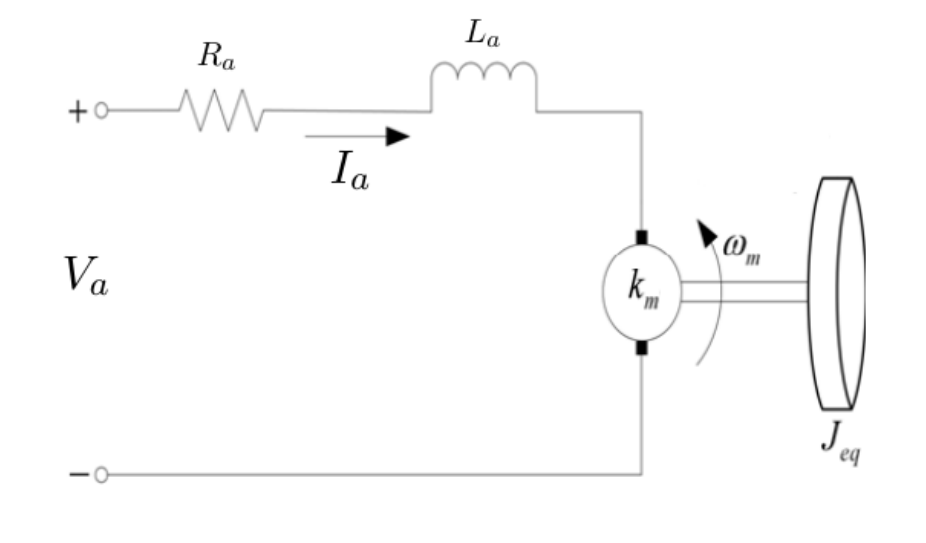
\includegraphics[scale=0.3]{circuito.png}
    \caption{Circuito}
\end{figure}

\quad O motor considerado tem as seguintes características dadas pelo fabricante:

\begin{itemize}[label={\textbullet}]
    \item Resistência de armadura: $R_a = 10.6 \Omega$
    \item Indutância de armadura: $L_a = 0.82 mH$
    \item Momento de Inércia do Rotor do Motor: $J_m = 1.16 \cdot  10^{-6} kgm^2$
    \item Constantes do Motor: $K_m = 0.0502 Nm/A$, $K_e = 0.0502 V s$
    \item Tensão máxima: 15 volts
    \item Massa do disco de inércia: $0.068 kg$
    \item Raio do disco de inércia: $0.0248 m$
\end{itemize}

\section{Modelagem teórica}

\quad Organizando as equações do sistema para obter o diagrama de blocos e a função de transferência.
Utilizando a Lei de Kirchhoff das Tensões, Equação do Torque, Lei do Motor e Lei do Gerador. Depois,
realizando a Transformada de Laplace das equações:

\begin{equation}
\begin{aligned}
    R_a \cdot i_a + L_a \frac{di_a}{dt} = V_a - e_c, \quad J_m \frac{d\omega_m}{dt} = T_m, \quad T_m = K_m \cdot i_a, \quad e_c = K_e \cdot \omega_m \\
    I_a(s) = \frac{1/R_a}{\frac{L_a}{R_a}s + 1}(V_a(s) - e_c(s)), \quad \Omega(s) = \frac{1}{J_m s }T_m(s), \quad T_m(s) = K_m \cdot I_a(s), \quad E_c(s) = K_e\Omega_m(s)
\end{aligned}
\end{equation}

\quad 1.1. Montando um diagrama de blocos do sistema (Desconsiderando o atrito do sistema).
O bloco azul é o subsistema elétrico, o bloco laranja é o subsistema mecânico e os blocos verdes são interligações entre o sistema elétrico e mecânico:

\begin{center}
\begin{tikzpicture}
 
    % Sum shape
    \node[draw,
        circle,
        minimum size=0.6cm,
        fill=white
    ] (sum) at (0,0){};
     
    \draw (sum.north east) -- (sum.south west)
        (sum.north west) -- (sum.south east);
     
    \draw (sum.north east) -- (sum.south west)
    (sum.north west) -- (sum.south east);
     
    \node[left=-1pt] at (sum.center){\tiny $+$};
    \node[below] at (sum.center){\tiny $-$};
     
    % corrente
    \node [draw,
        fill=cyan,
        minimum width=2cm,
        minimum height=1.2cm,
        right=1cm of sum
    ]  (corrente) {$\frac{1/R_a}{\frac{L_a}{R_a}s + 1}$};

    % torque
    \node [draw,
        fill=lime,
        minimum width=2cm,
        minimum height=1.2cm,
        right=1cm of corrente
    ]  (torque) {$K_m$};
     
    % velocidade
    \node [draw,
        fill=orange, 
        minimum width=2cm, 
        minimum height=1.2cm,
        right=1cm of torque
    ] (velocidade) {$\frac{1}{J_m s}$};
     
    % eletromotriz
    \node [draw,
        fill=lime, 
        minimum width=2cm, 
        minimum height=1.2cm, 
        below right= 1cm and -2cm of torque
    ]  (eletromotriz) {$K_e$};
     
    % Arrows with text label
    \draw[-stealth] (sum.east) -- (corrente.west);

    \draw[-stealth] (corrente.east) -- (torque.west) 
        node[midway,above]{$I_a$};
     
    \draw[-stealth] (torque.east) -- (velocidade.west) 
        node[midway,above]{$T_m$};
     
    \draw[-stealth] (velocidade.east) -- ++ (1.25,0) 
        node[midway](output){}node[midway,above]{$\Omega_m$};
     
    \draw[-stealth] (output.center) |- (eletromotriz.east);
     
    \draw[-stealth] (eletromotriz.west) -| (sum.south) 
        node[near end,left]{$E_c$};
     
    \draw (sum.west) -- ++(-1,0) 
        node[midway,above]{$V_a$};
     
\end{tikzpicture}
\end{center}

\quad 1.2. Calculando a função de transferência do motor $G(s)$ de $V_a(s)$ para $\Omega_m(s)$
(Levando em consideração que é um sistema realimentado):

\begin{equation}
    G(s) = \frac{\Omega_m(s)}{V_a(s)}
    = \frac{\frac{K_m}{R_a \cdot J_m}\frac{1}{s (\frac{L_a}{R_a}s + 1)}}{1 + \frac{K_e \cdot K_m}{R_a \cdot J_m}\frac{1}{s (\frac{L_a}{R_a}s + 1)}}
    = \frac{k_m}{R_a \cdot J_m \cdot s \cdot (\frac{L_a}{R_a}s + 1) + K_e \cdot K_m}
    = \frac{\frac{k_m}{J_m \cdot L_a}}{s^2 + \frac{R_a}{L_a}s + \frac{K_e \cdot K_m}{J_m \cdot L_a}}
\end{equation}

\quad 1.3. Representando o sistema no espaço de estados com a realização canónica controlável:

\begin{equation}
\begin{aligned}
    \dot{x} =
    \begin{bmatrix}
        0 && 1 \\
        -\frac{K_e \cdot K_m}{J_m \cdot L_a} && -\frac{R_a}{L_a}
    \end{bmatrix}
    +
    \begin{bmatrix}
        0 \\
        1
    \end{bmatrix}
    u \\
    y =
    \begin{bmatrix}
        \frac{k_m}{J_m \cdot L_a} && 0
    \end{bmatrix}
\end{aligned}
\end{equation}

\end{document}